\documentclass[UTF8,a4paper]{ctexart}
\usepackage[utf8]{inputenc}
\usepackage{amsmath}
\usepackage{pdfpages}
\usepackage{graphicx}
\usepackage{wrapfig}
\usepackage{listings}
\usepackage{multicol}
\newcommand{\tabincell}[2]{\begin{tabular}{@{}#1@{}}#2\end{tabular}}
\title{实验一\ \ 单管放大电路仿真及实验}
\author{张蔚桐\ 2015011493\ 自55}
\begin {document}
\maketitle
\section{预习任务}
\subsection{JFET管的输入特性和传输特性的测试}
\begin{wrapfigure}{r}{0pt}
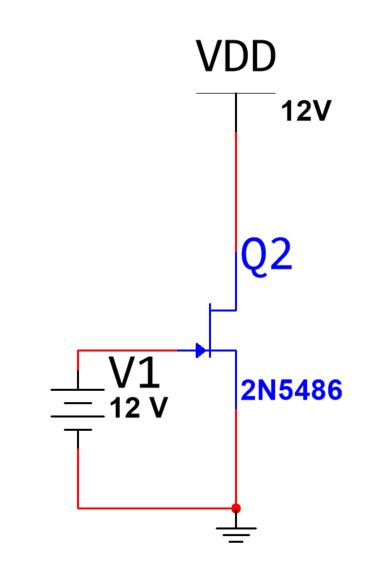
\includegraphics [width=30mm]{in.jpg}
\caption{输入特性测试电路}
\label{cin}
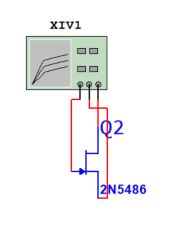
\includegraphics [width = 30mm]{transfer.jpg}
\caption{传输特性测试电路}
\label{ctransfer}
\end{wrapfigure}
如图\ref{cin}所示是N沟道型JFET管2N5486的输入特性测试电路图,对$V_1$进行直流参数仿真,可以得到如图\ref{in}的仿真图像。

从图像可以得到,JFET的$U_{GS(off)}\approx-3.772\rm{V}$

如图\ref{ctransfer}所示是2N5486的传输特性测试电路图,仿真时将IV测试仪选择为NMOS管测量模式,可以得到如图\ref{transfer}的仿真图像
其中,对图像静态工作点附近进行进一步细致的仿真可以得到如图\ref{micro}所示的图像,其中,三条曲线分别为$V_{gs}=-2.222,-2.778,-3.333\rm{V}$时的特性图

因此,可以得到2N5486的$I_{dss}=14.4648mA,1.4<g_m<2.4(mA/V^2)$,其中$g_m$的变化比较大,收仿真条件的限制只能给出近似的值
\begin{figure}
\centering 
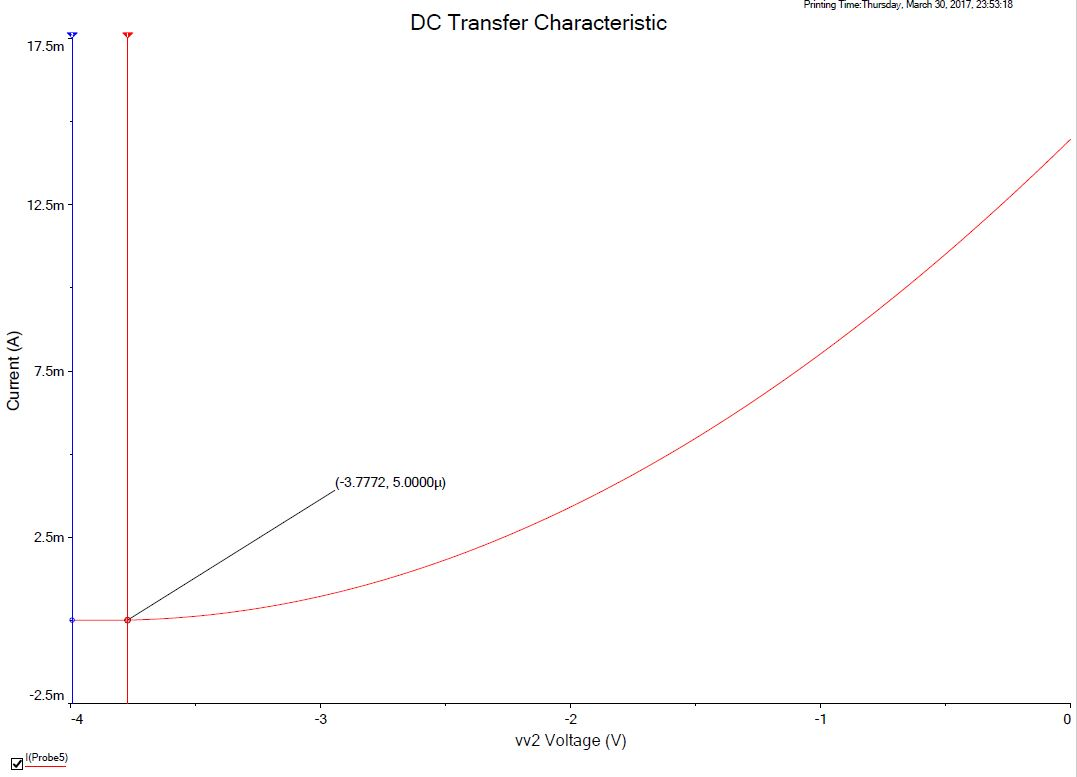
\includegraphics[width=\textwidth]{ugsoff.jpg}
\caption{2N5486输入特性曲线}
\label{in}
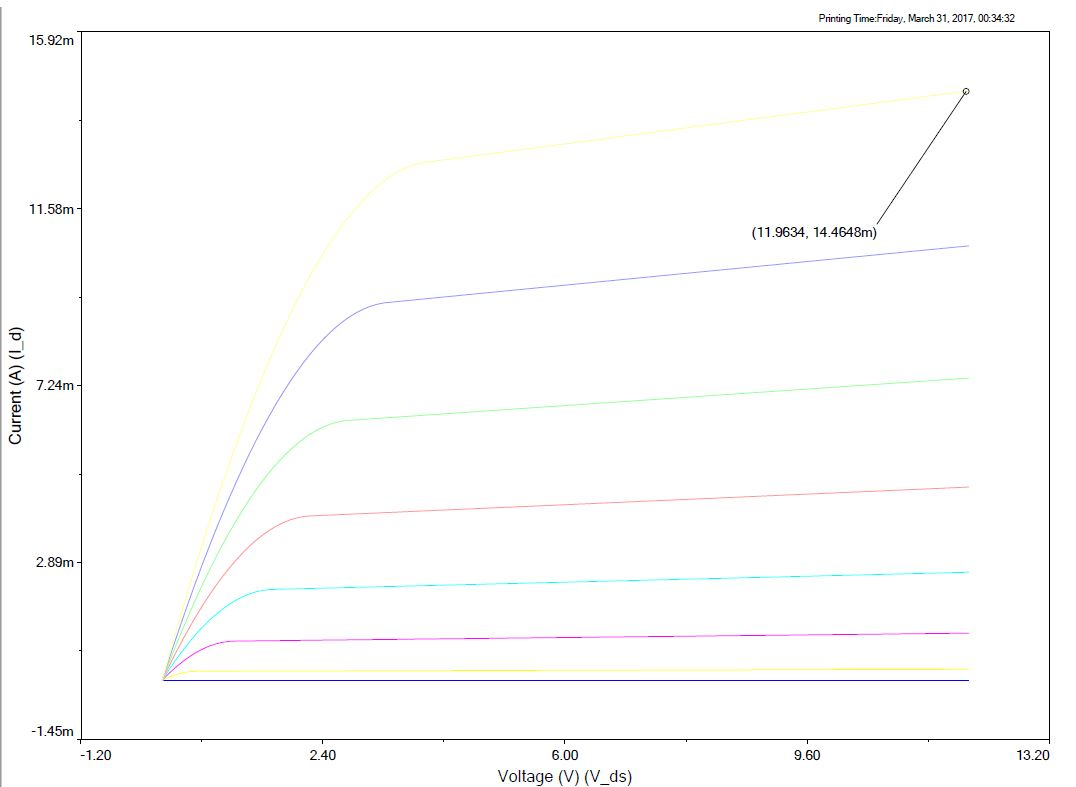
\includegraphics[width=\textwidth]{ids.jpg}
\caption{2N5486传输特性曲线}
\label{transfer}
\end{figure}
\begin{figure}
\centering
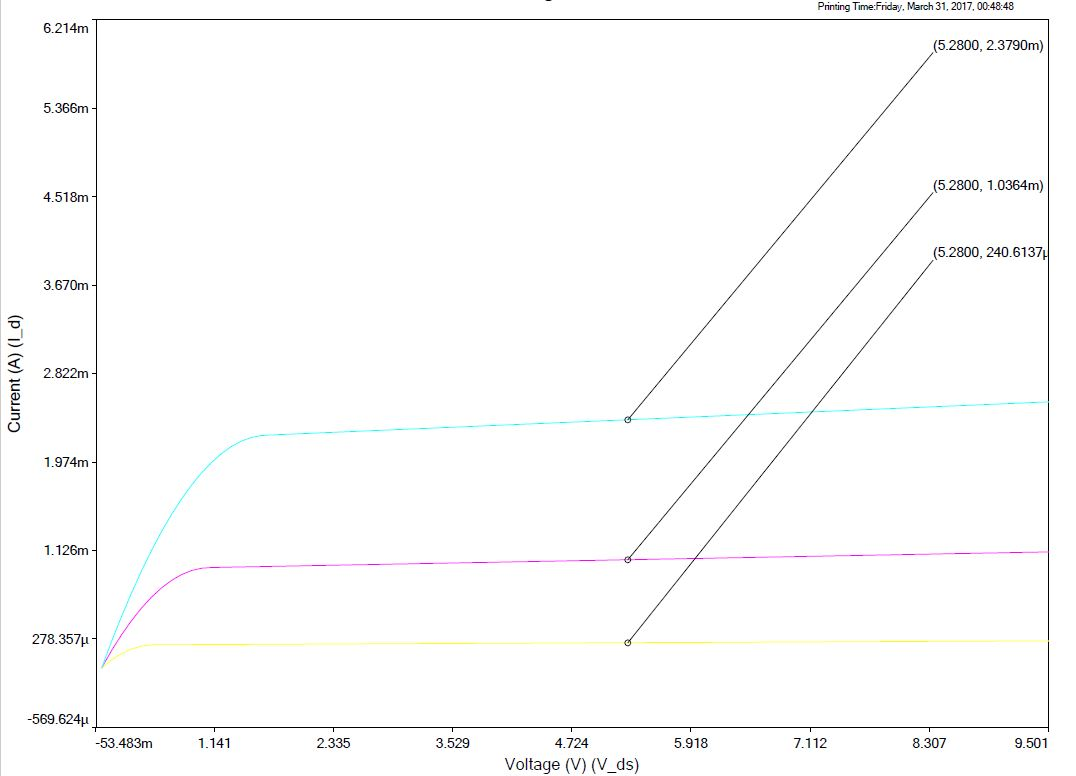
\includegraphics[width=\textwidth]{gm.jpg}
\caption{工作点附近的$g_m$的测量}
\label{micro}
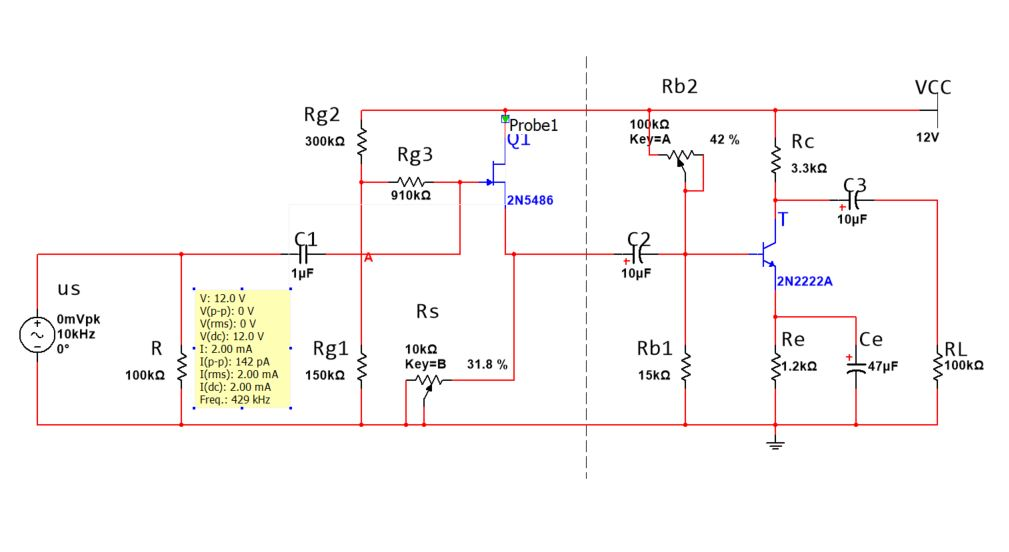
\includegraphics [width=\textwidth]{vII.jpg}
\caption{(两级)放大电路电路图}
\label{vi}
\end{figure}
\clearpage
\subsection{JFET单管CD电路的理论计算和仿真}
\subsubsection{静态参数的设置}
如图\ref{vi}所示是已经搭建好的两级放大电路图,其中后级电路采用第一次实验中使用9011搭建的CE电路(这里使用2N2222A代替9011)。
实验电路参数满足$I_{CQ}=2\rm{mA}$。具体的参数实现在上次实验中已经经过了理论计算和验证了,这里从略

这里着重分析前级电路的静态工作情况。首先可以近似得到$U_a=3V$实验要求$I_{DQ}=2mA$因此可以得到$$I_{DQ}=\frac{I_{DSS}}{U_{GS(\rm{off})}^2}((3-I_{DQ}R_s)^2-U_{GS(\rm{off})}^2)$$
可以解得$R_s=3.512\mathrm{k}\Omega$

和图\ref{vi}的仿真结果$R_s=3.18\mathrm{k}\Omega$相差不大
\subsubsection{动态参数的测试}
显然,电路的输入电阻$R_i\approx100\mathrm{k}\Omega$如图\ref{ri}所示,电路测量电阻约为91$\mathrm{k}\Omega$,和估算值相近

根据CD电路的基本知识,我们可以得到$\displaystyle{A_u=\frac{g_mR_s}{1+g_mR_s}=0.88}$如图\ref{A1}所示,可以测得仿真值大约为0.91,和计算得到的值相近
\begin{figure}
\centering
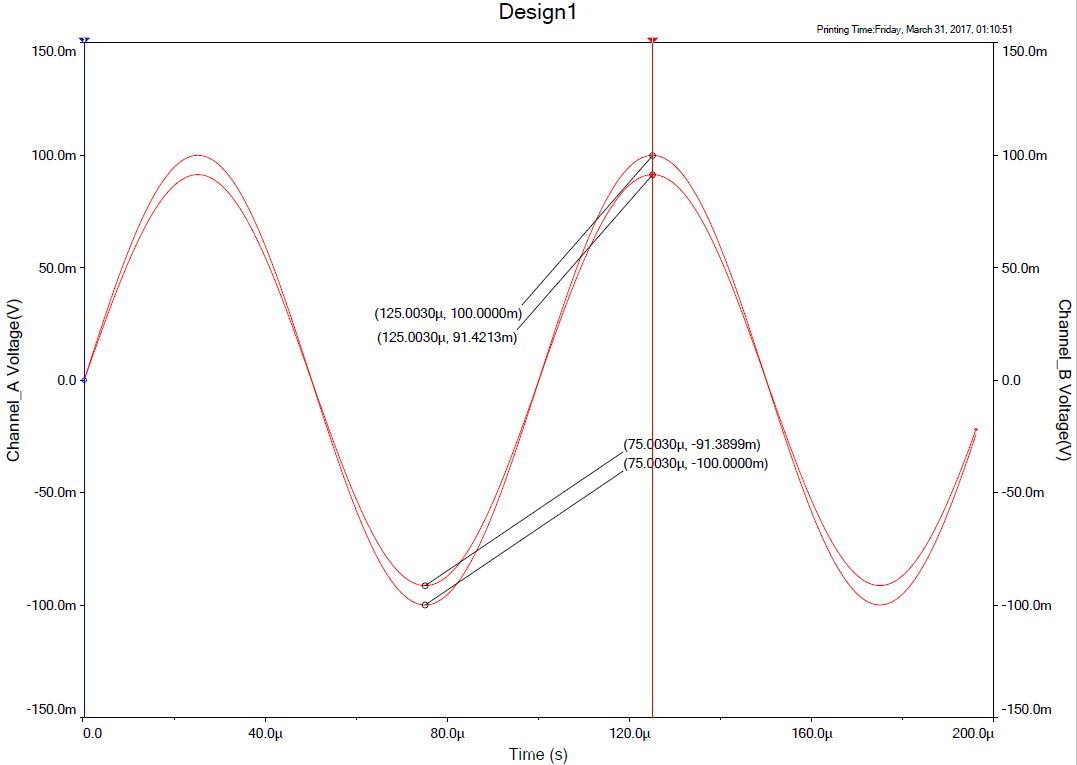
\includegraphics[width=\textwidth]{AA.jpg}
\caption{单级CD电路的电压放大参数}
\label{A1}
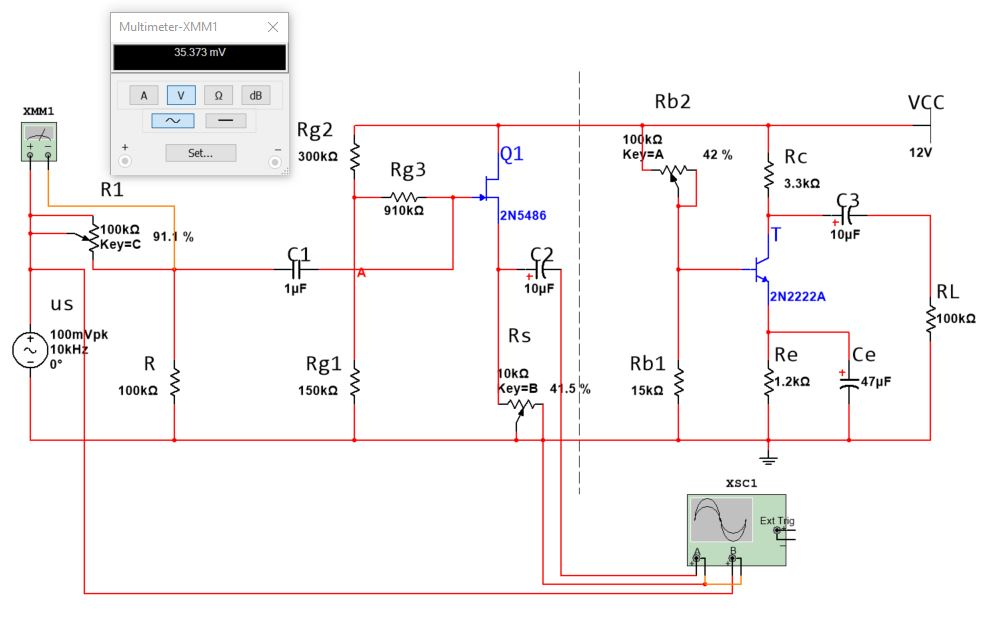
\includegraphics [width=\textwidth]{Ri.jpg}
\caption{单级CD电路的输入电阻}
\label{ri}
\end{figure}
\subsection{两级放大电路的搭建和仿真}
同上节,图\ref{vi}所示是已经搭建好的两级放大电路图,根据之前的实验分析可以直接得到$R_i=100\mathrm{k}\Omega,R_o=3.3\mathrm{k}\Omega$而图\ref{ri1},\ref{ro1}是他们的仿真电路,仿真测得$R_i=91\mathrm{k}\Omega,R_o=3.08\mathrm{k}\Omega$和理论计算基本相近

CD电路电路下面讨论两级电路放大系数的问题,我们估计三极管$\beta=220,r_{be}=3\mathrm{k}\Omega$并设CD电路$U_gs=U$可以得到:
\begin{equation}\begin{aligned}
&U_i=U+g_mU(R_s//R_{b1}//R_{b2}//r_{be}) \\ 
&U_o=\frac{\beta R_cg_mU(R_s//R_{b1}//R_{b2}//r_{be})}{r_{be}}\\
&A=\frac{\beta R_cg_m(R_s//R_{b1}//R_{b2}//r_{be})}{r_{be}}/(1+g_m(R_s//R_{b1}//R_{b2}//r_{be}))=184
\end{aligned}\end{equation}
如图\ref{AAAA}仿真可得电路放大系数为168,误差可以接受
\begin{figure}
\centering
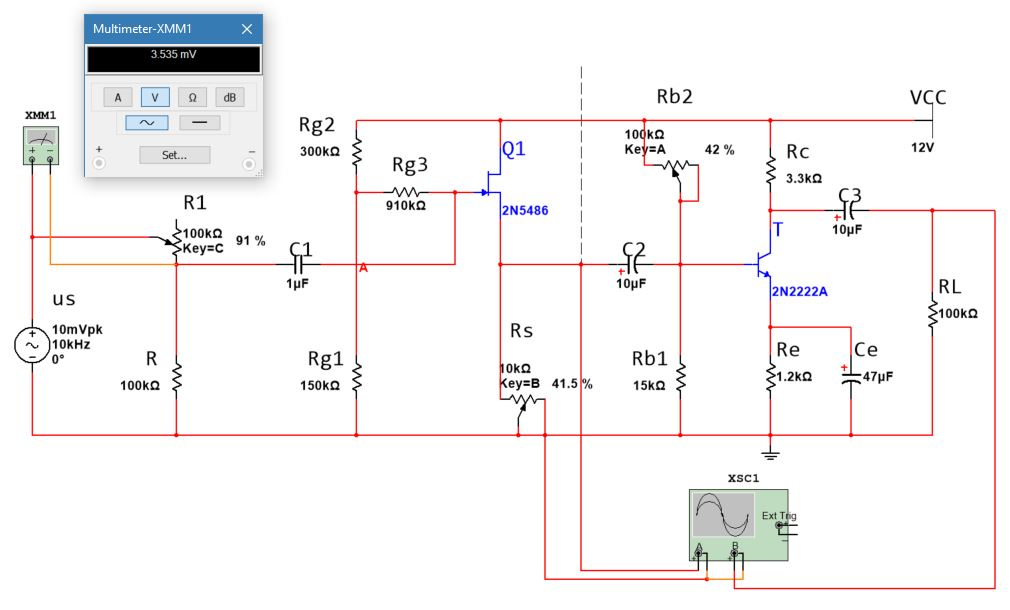
\includegraphics[width=\textwidth]{Ri2.jpg}
\caption{两级放大电路的输入电阻测试图}
\label{ri1}
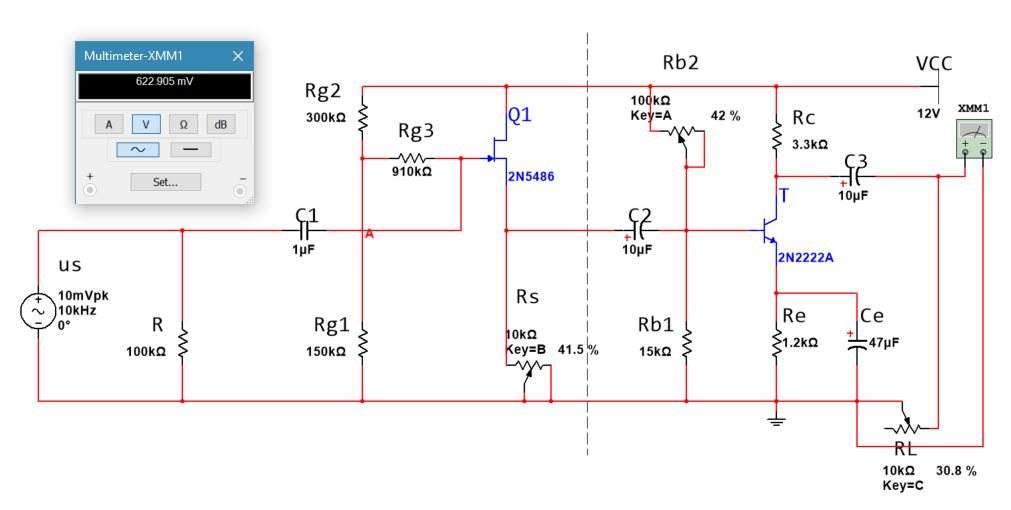
\includegraphics [width=\textwidth]{Ro2.jpg}
\caption{两级放大电路的输出电阻测试图}
\label{ro2}
\end{figure}.
\begin{figure}
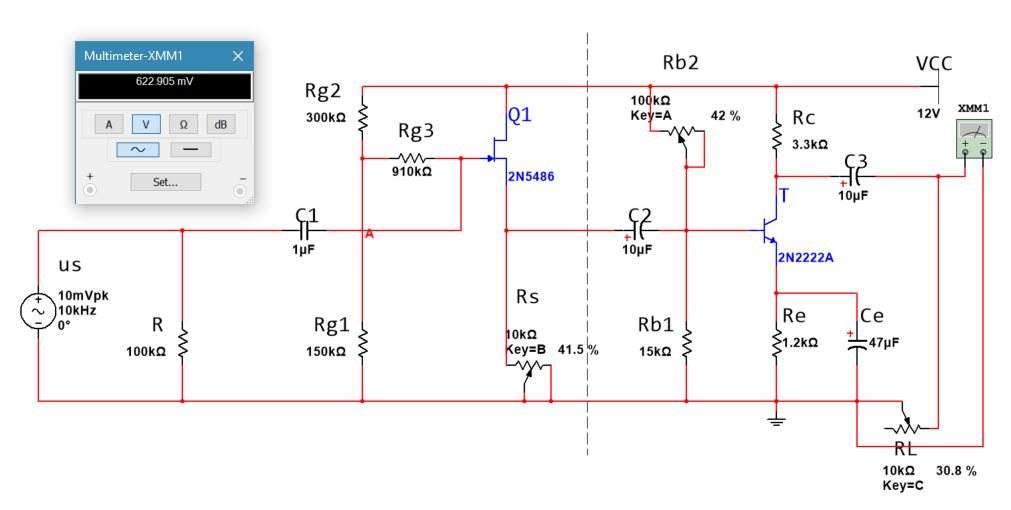
\includegraphics [width=\textwidth]{Ro2.jpg}
\caption{两级放大电路的放大系数测试图}
\label{ro2}
\end{figure}
\section{实验数据记录}
\end{document}
